

%\author[Niklas Brunn]{Nix}


\beamertemplatenavigationsymbolsempty{}

\logo{
\includegraphics[height=1cm]{Bilder/logo}}

%\begin{frame}
%\frametitle{Summary}
%\tableofcontents
%\end{frame}


\section{Formulation of the optimization problem}

   \subsection{Unconstrained NLP}
   
   \begin{frame}
   \frametitle{Unconstrained NLP}
   \begin{itemize}
   	\item[] $$\argmin_{\theta\in\mathbb{R}^{d}}\quad f_{\mathrm{M}}(\theta)$$
   	\pause
   	\item $\theta$ decision variables and $d$ dimension of parameter space
    \pause
   	\item objective function
   	$$f_{\mathrm{M}}(\theta) := \frac{1}{N}\sum_{(x, y)\in\mathrm{M}}^{}\mathrm{L}_{y}(\text{akt}_{(.)}(\mathrm{R}_{x}(\theta)))$$
   	%(empirical risk of the DNN with current parameters $\theta$ given the subdataset $\mathrm{M}$);
   	\pause
   	\item $\mathrm{M}\subset\mathrm{D} := \{(x_{i}, y_{i})_{1\leq i\leq N}\}$ observation data;\\ 
   	$\mathrm{R}_{x}(\theta)$ realisation of a DNN given the observed value $x$ with current parameters $\theta$;\\
   	$\text{akt}_{(.)}(\hat{y}) := \left(akt(\hat{y}_{1}), \ldots, akt(\hat{y}_{1})\right)$ elementwise application of a convex activation function on the vector $\hat{y}$;\\
   	$\mathrm{L}_{z} := \text{Loss}(z, y)$ non-decreasing, convex loss function in $z$\\ given the target $y$
   \end{itemize}
  \end{frame}
   
   
   
   %\begin{frame}
   %\frametitle{Example graphics}
   %\begin{figure}[h!]
   %		\centering
   %		\includegraphics[scale=0.43, trim= 110mm 0mm 0mm 0mm]{Bilder/NeuralODE}
   %	\end{figure}
   %\end{frame}

   \subsection{Optimization method}
  
  \subsection{Implementation}
  

   %\begin{frame}
   %\frametitle{SDE Beispiele}
   %\begin{tiny}SDE-Pfad-Simulationen von Ben Deitmar\end{tiny}
   %\begin{figure}[h!]
   %\begin{minipage}{0.4\textwidth}
   %		%\begin{mdframed}[style=innersmall]
   %		\center{}
   %		\includegraphics[scale=0.27]{Bilder/SDE_sig=0}
   %		\begin{tiny} $\mathrm{d}X_{t}=X_{t}\text{ }\mathrm{d}t+0\text{ }\mathrm{d}W_{t},$ $X_{0}=1$\\ $\mathrm{d}X_{t}=X_{t}\text{ }\mathrm{d}t+0\text{ }\circ \mathrm{d}W_{t},$ $X_{0}=1$ \end{tiny}
   %		\center{}
   %		\includegraphics[scale=0.27]{Bilder/SDE_BB}
   %		\begin{tiny} $\mathrm{d}X_{t}=0\mathrm{d}t+\mathrm{d}W_{t},$ $X_{0}=1$\\ $\mathrm{d}X_{t}=0\mathrm{d}t+\circ\mathrm{d}W_{t},$ $X_{0}=1$\end{tiny}
   		%\center{}
   		%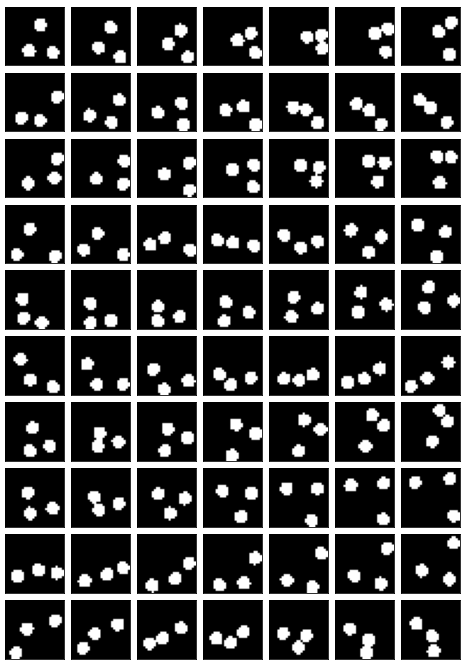
\includegraphics[scale=0.15]{Bilder/bouncingBalls_ODEorig2}
   		%\end{mdframed}
   %	\end{minipage}
   %\begin{minipage}{0.4\textwidth}
   		%\begin{mdframed}[style=innersmall]
   %		\center{}
   %		\includegraphics[scale=0.27]{Bilder/SDE_mu=x_sig=tt}
   %		\begin{tiny} $dX_{t}=X_{t}\text{ }\mathrm{d}t+t^{2}\text{ }\mathrm{d}W_{t},$ $X_{0}=1$\\
   %		$dX_{t}=X_{t}\text{ }\mathrm{d}t+t^{2}\text{ }\circ\mathrm{d}W_{t},$ $X_{0}=1$\end{tiny}
   		%\center{}
   		%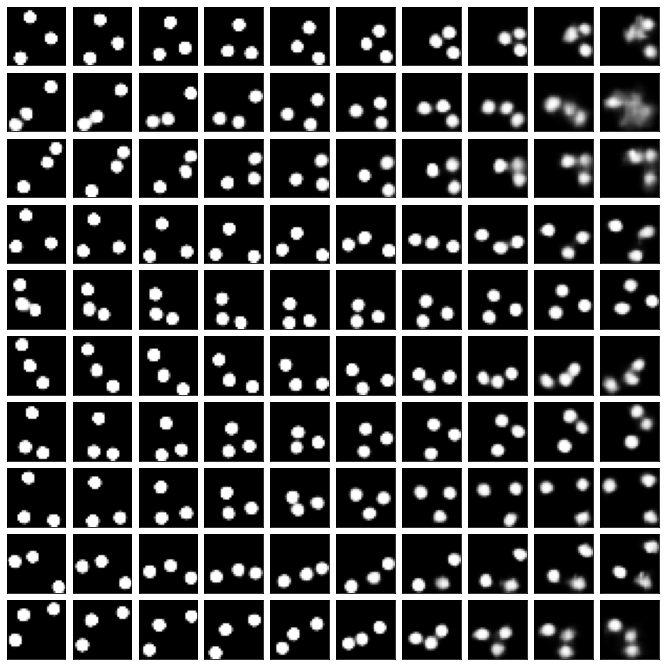
\includegraphics[scale=0.15]{Bilder/bouncingBalls_ODE}
   		%\end{mdframed}
   	%\end{minipage}
   %\begin{minipage}{0.2\textwidth}
   	%\begin{mdframed}[style=innersmall]
   	%\center{}
   	%\includegraphics[scale=0.27]{Bilder/SDE_mu=x_sig=tt_x0=0}
   	%\begin{tiny} $dX_{t}=0+X_{t}\text{ }\mathrm{d}t+t^{2}\text{ }\mathrm{d}W_{t},$ $X_{0}=0$\\ $dX_{t}=0+X_{t}\text{ }\mathrm{d}t+t^{2}\text{ }\circ\mathrm{d}W_{t},$ $X_{0}=0$\end{tiny}
   	%\center{}
   	%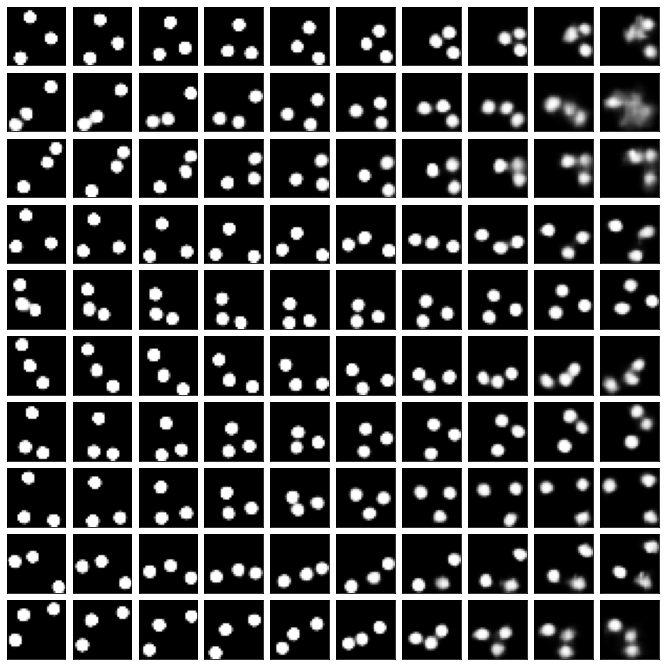
\includegraphics[scale=0.15]{Bilder/bouncingBalls_ODE}
   	%\end{mdframed}
  % \end{minipage}
  % \end{figure}
%\end{frame}




 
 
\section{Experiments}   

\subsection{Simple simulated dataset}

\subsection{MNIST}

